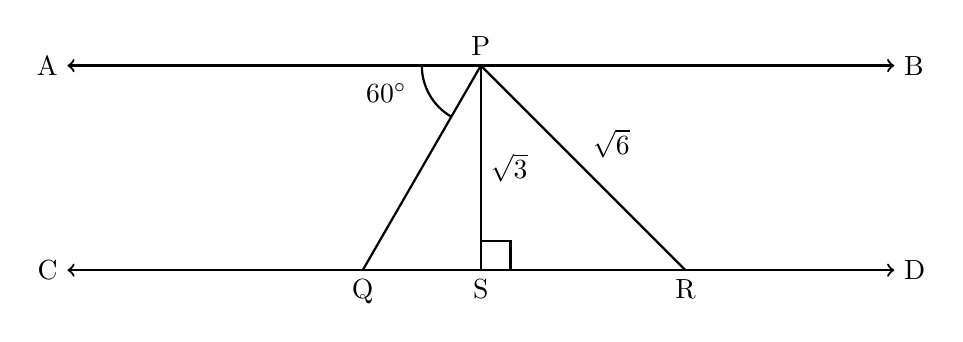
\begin{tikzpicture}[scale=1.5]

    % --- Define Coordinates based on geometric properties ---
    % Assume height PS = sqrt(3) ~ 1.732
    % Then triangle PQS is a 30-60-90 triangle.
    % Angle SPQ = 30, Angle PQS = 60.
    % Base QS = PS / tan(60) = sqrt(3)/sqrt(3) = 1.
    % So if S is (0,0), P is (0, 1.732), Q is (-1, 0).
    %
    % For triangle PSR:
    % Hypotenuse PR = sqrt(6). Height PS = sqrt(3).
    % Base SR = sqrt( (sqrt(6))^2 - (sqrt(3))^2 ) = sqrt(3) ~ 1.732.
    % So R is at (1.732, 0).

    \coordinate (S) at (0,0);
    \coordinate (P) at (0, 1.732); % sqrt(3)
    \coordinate (Q) at (-1, 0);
    \coordinate (R) at (1.732, 0); % sqrt(3)

    % Define endpoints for the parallel lines
    \coordinate (A_end) at (-3.5, 1.732);
    \coordinate (B_end) at (3.5, 1.732);
    \coordinate (C_end) at (-3.5, 0);
    \coordinate (D_end) at (3.5, 0);

    % --- Draw Parallel Lines (Rays/Lines with arrows) ---
    % Top line AB
    \draw[<->, thick] (A_end) -- (B_end);
    % Bottom line CD
    \draw[<->, thick] (C_end) -- (D_end);

    % --- Draw Triangle Segments ---
    \draw[thick] (P) -- (Q); % Segment PQ
    \draw[thick] (P) -- (S); % Segment PS (Altitude)
    \draw[thick] (P) -- (R); % Segment PR

    % --- Labels for Points ---
    \node[left] at (A_end) {A};
    \node[right] at (B_end) {B};
    \node[left] at (C_end) {C};
    \node[right] at (D_end) {D};
    
    \node[above] at (P) {P};
    \node[below] at (Q) {Q};
    \node[below] at (S) {S};
    \node[below] at (R) {R};

    % --- Labels for Measurements ---
    % Label for height PS
    \node[right] at (0, 0.866) {$\sqrt{3}$};
    
    % Label for hypotenuse PR
    \node[above right] at (0.866, 0.866) {$\sqrt{6}$};

    % --- Angle Arc and Label ---
    % Angle at P (between line PA and segment PQ)
    % Line PA is angle 180. Segment PQ is angle 240 (from P).
    % We draw arc from 180 to 240.
    \draw[thick] (P) + (180:0.5cm) arc (180:240:0.5cm);
    \node at (-0.8, 1.5) {$60^{\circ}$};

    % --- Right Angle Symbol ---
    % At point S, between PS (up) and SR (right)
    \draw[thick] (0, 0.25) -- (0.25, 0.25) -- (0.25, 0);

\end{tikzpicture}